\documentclass[11pt, titlepage]{article}
\usepackage{amsmath,amsthm,amssymb}
\usepackage{hyperref, pgf, tikz}
\usepackage{fancyhdr}
\usetikzlibrary{arrows}
\usepackage[margin=1.25in]{geometry}
\usepackage{graphicx}                     
\pagestyle{fancy}
\usepackage{array}

\lhead{Lab \#1}
\rhead{\thepage}
\cfoot{}

\title{Newton's Second Law: The Atwood Machine \\ \ \\ \large Lab \#1}
\author{Name: Avery Karlin \\ Partner: Alon Levin}
\date{}
\begin{document}

\maketitle

\begin{center}
\LARGE Newton's Second Law: The Atwood Machine
\end{center}

\section*{Objective}
The objective of the lab is to measure the acceleration of an Atwood pulley machine for varying total masses and forces, while keeping the other measure constant.
\section*{Introduction}
The main theory used within the lab is that of Newton's Second Law: $$F_{net} = ma,$$ such that within an Atwood machine, or two masses on opposite sides of a pulley, the force of gravity, $F_g = mg$, works in opposite directions. Since the pulley is all joined together, the total acceleration of the system is constant. In addition, due to the real world constraints, we must also subtract the force of friction (both from the pulley and from the surrounding air), and add the mass of the pulley to the total mass.

Thus, $F_{net} = (m_1 + m_2 + m_{pulley})a = m_1g - m_2g - f$, where f is the force of friction. This can then be rewritten as $$a = \frac{m_2 - m_1)g - f}{m_1 + m_2 + m_{pulley}}.$$ This can then be taken when a = 0, such that the frictional force of the system, divided by the gravitational constant to find the mass that must be subtracted out due to friction: $$a = \frac{(m_2 - m_1 - m_f)g}{m_1 + m_2 + m_{pulley}}.$$

The acceleration of the actual experimental system is done through determining the time the mass takes to fall a specific distance, such that the equation, $$y = v_0t + \frac{1}{2}at^2,$$ can be used to find the acceleration of the system, assuming it is constant. It can then be modified due to starting from rest, solving for acceleration to: $$a = \frac2y}{t^2}.$$
\section*{Procedures and Results}

\begin{figure}[t]
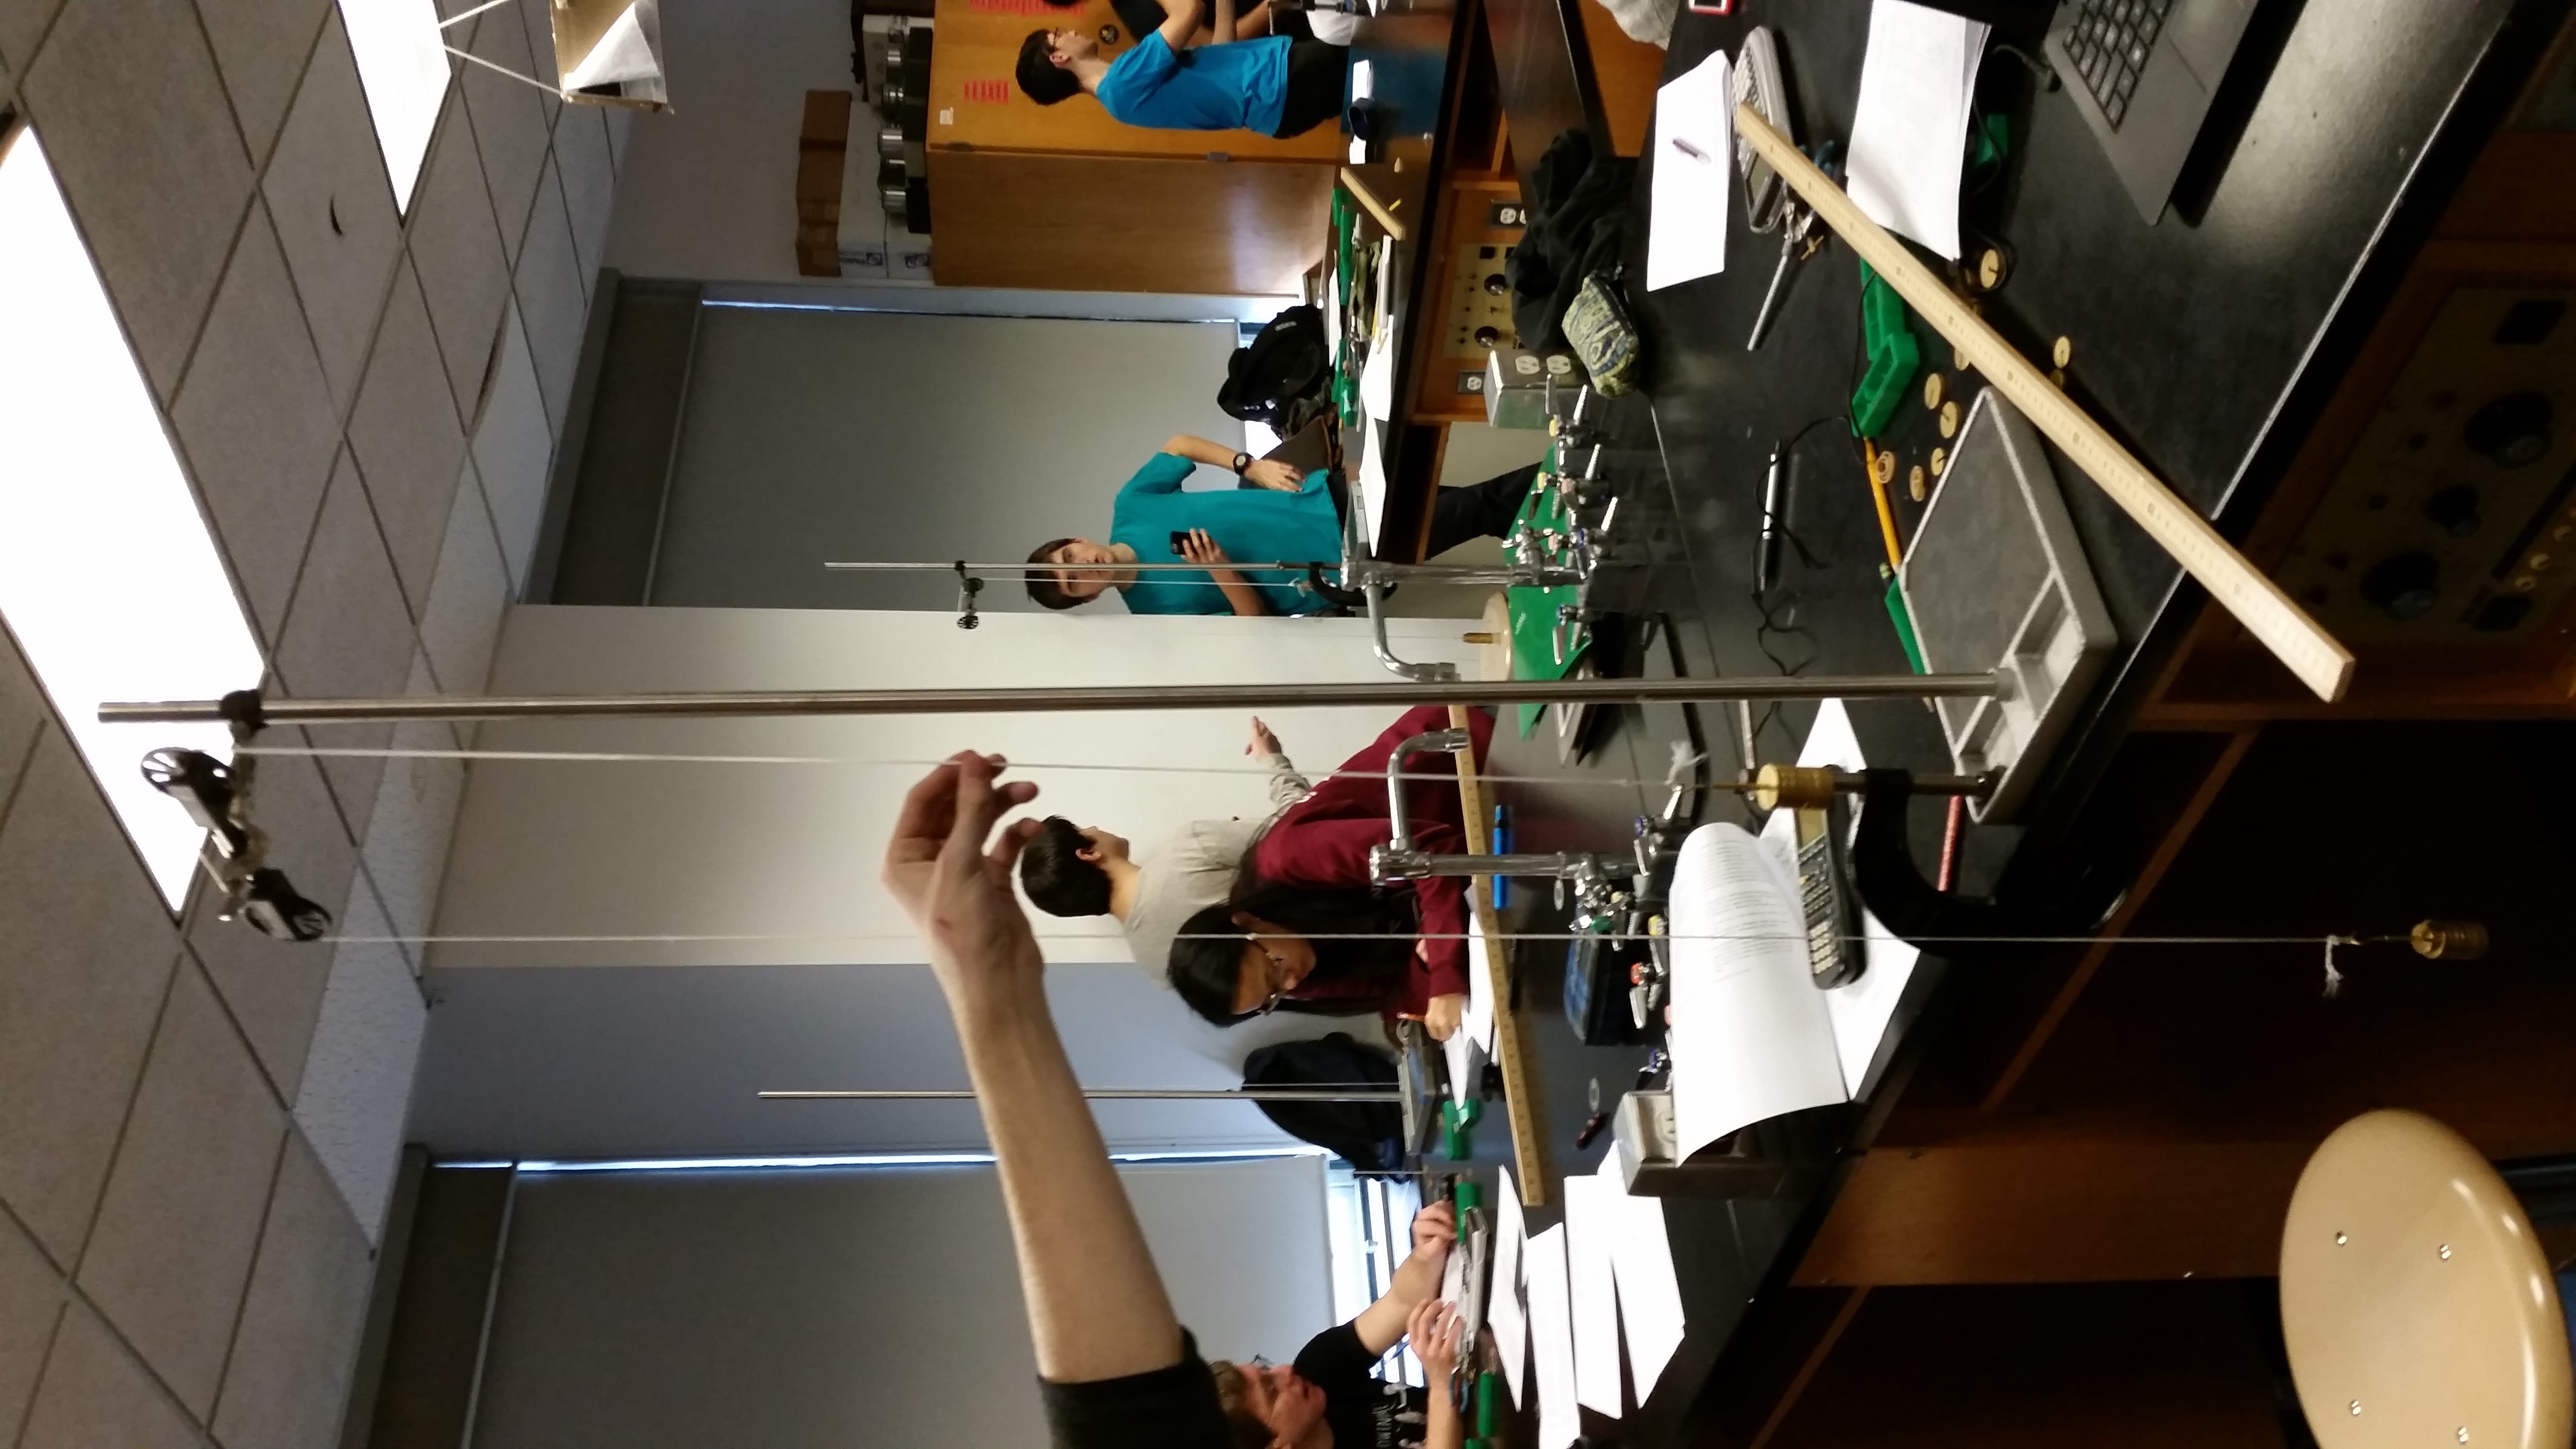
\includegraphics[scale=0.1, angle=270]{lab1.jpg}
\end{figure}

First, the entire Atwood machine setup must be built, with equal masses on both sides, adding mass to one side until a = 0, such that the added mass is $m_f$, the mass needed to compensate for friction, then we added mass to the descending side, and measuring the amount of time it took to fall a specific distance. After, we tested using different masses on both, but preserving the relative mass,  creating different frictional masses/forces on each, measuring the resultant acceleration.

Next, 

\begin{center}
$$m_{eq} = 31.6 g$$
\begin{tabular}
{|m{7em}|m{7em}|m{7em}|m{7em}|m{7em}|}
\hline
Trial & 1 & 2 & 3 & 4 \\
\hline
Descending Mass, $m_2$ (kg) & 0.06636 & 0.165 & & \\
\hline
Ascending Mass, $m_1$ (kg) & 0.055 & 0.150 & & \\
\hline
Distance of Travel, $y$ (m) & 0.8984 & 0.855 & & \\
\hline
Time of Travel, Run 1, $t_1$ (s) & 1.47 & 2.1 & & \\
\hline
Time of Travel, Run 2, $t_2$ (s) & 1.21 & 2.27 & & \\
\hline
Time of Travel, Run 3, $t_3$ (s) & 1.31 & 2.18 & & \\
\hline
Average Time, $t_{avg}$ (s) & 1.33 & 2.183 & & \\
\hline
Measured Acceleration, $a_m$ ($kgm/s^2$) & 1.015 & & & \\
\hline
Total Mass, $m_t$ (kg) & 0.1529 & & & \\
\hline
Frictional Mass, $m_f$ (kg) & 0.00136 & 0.005 & & \\
\hline
Net Force, $F_{net}$ (N) & 0.098 & & & \\ 
\hline
Theoretical Acceleration, $a_t$ ($kg*m/s^2$) & 0.64 & & & \\
\hline
Percent Acceleration Error (\%) & 58.59 & & & \\
\hline
\end{tabular}
\begin{tabular}
{|m{7em}|m{7em}|m{7em}|m{7em}|m{7em}|}
\hline
Trial & 5 & 6 & 7 & 8 \\
\hline
Descending Mass, $m_2$ (kg) & & & & \\
\hline
Ascending Mass, $m_1$ (kg) & & & & \\
\hline
Distance of Travel, $y$ (m) & & & & \\
\hline
Time of Travel, Run 1, $t_1$ (s) & & & & \\
\hline
Time of Travel, Run 2, $t_2$ (s) & & & & \\
\hline
Time of Travel, Run 3, $t_3$ (s) & & & & \\
\hline
Average Time, $t_{avg}$ (s) & & & & \\
\hline
Measured Acceleration, $a_m$ ($kgm/s^2$) & & & & \\
\hline
Total Mass, $m_t$ (kg) & & & & \\
\hline
Frictional Mass, $m_f$ (kg) & & & & \\
\hline
Net Force, $F_{net}$ (N) & & & & \\ 
\hline
Theoretical Acceleration, $a_t$ ($kg*m/s^2$) & & & & \\
\hline
Percent Acceleration Error (\%) & & & & \\
\hline
\end{tabular}

\end{center}

\section*{Discussion}
Sample calculations for the non-measured data are as shown:
$$t_{avg} = \frac{t_1 + t_2 + t_3}{3} = \frac{1.47 + 1.21 + 1.31}{3} = 1.33$$
$$a = \frac{2y}{t^2} = \frac{2*0.8984}{1.33^2} = 1.015$$
$$m_t = m_1 + m_2 + m_{pulley} = 0.06636 + 0.055 + 0.0316 = 0.1529$$
$$F_{net} = (m_2 - m_1 - m_f)g = (0.06636 - 0.055 - 0.00136)(9.8) = 0.098$$
$$a_t = \frac{F_{net}}{m_t} = \frac{0.098}{0.1529} = 0.64$$
$$\text{Percent Acceleration Error} = \frac{|a_t - a_m|}{a_t}*100\% = \frac{|0.64 - 1.015|}{0.64}*100\% = \frac{0.375}{0.64}*100\% = 58.59\%$$

\section*{Conclusion}

\end{document}
